\documentclass[dvipdfmx,platex]{beamer}
\usetheme{metropolis}% Use metropolis theme
\usepackage{booktabs}
\usepackage[deluxe]{otf}% 多書体設定を使う
\usepackage[labelformat=empty]{caption}
% \renewcommand{\kanjifamilydefault}{gt}
\title{{\mgfamily 機械学習勉強会 第1回}}
\date{June 13, 2017}
\author{{\mgfamily 中村 遼太郎}}
\institute{}
\begin{document}
\mgfamily
\maketitle
\begin{frame}{Table of contents}
  \setbeamertemplate{section in toc}[sections numbered]
  % \tableofcontents[hideallsubsections]
  % 分類が変
  Supervised Learning
  \tableofcontents[part=1]
  Unsupervised Learning
  \tableofcontents[part=2]
\end{frame}
\begin{frame}[fragile]{{\mgfamily 今日の目標}}
  次回以降に学ぶアルゴリズムと例題の概要を知る
  \begin{table}
    \caption{{\mgfamily アルゴリズムと適用例}}
    \begin{tabular}{@{} ll @{}}
      \toprule
      アルゴリズム & 適用例\\
      \midrule
      分類 & スパムメール判定\\
      回帰分析 & 売上予測\\
      クラスタリング & 画像の減色処理\\
      \bottomrule
    \end{tabular}
  \end{table}
\end{frame}
\part{Supervised Learning}
\begin{frame}{パラメトリック法}
  モデル(数式)を仮定し,モデルの最適なパラメタを学習する
  % \vspace{20pt}
  \begin{columns}[T,onlytextwidth]
    \column{0.50\textwidth}
    パラメトリック法の手順
    \begin{enumerate}
    \item データの予測モデルを仮定
    \item モデルのパラメタの評価基準を決める
    \item パラメタを決める
    \end{enumerate}
    \column{0.50\textwidth}
    \begin{figure}
      \centering
      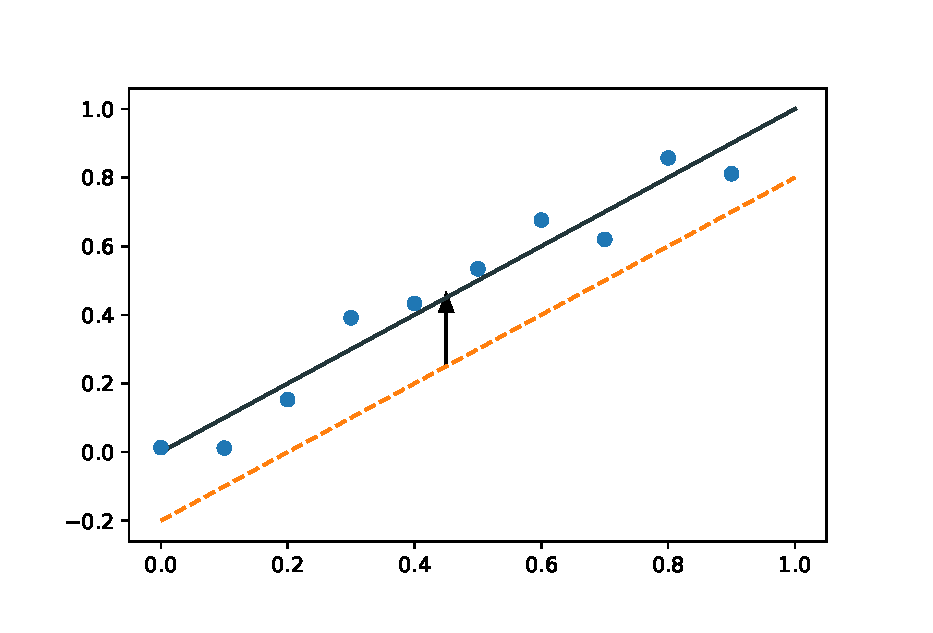
\includegraphics[width=5cm]{fig/arrange_params.eps}
      \caption{{\mgfamily 一次関数のモデルのパラメタ調整}}
    \end{figure}
  \end{columns}
\end{frame}
\section{Classification}
\begin{frame}{分類}
  クラスに分類された既存データを元に新規データを分類する
\end{frame}
\section{Perceptron}
\begin{frame}{パーセプトロン, モデル}
  線形モデル$f$を設定する
\end{frame}
\begin{frame}{パーセプトロン, 評価基準}
  誤分類の度合$E$が最小になる$w_i$を求める
\end{frame}
\begin{frame}{ロジスティック回帰, モデル}
  パーセプトロンと同じく線形モデル$f$を設定する
\end{frame}
\begin{frame}{ロジスティック回帰, モデル}
  ただし,$|f|$が大きいほど$t$である確率が高いとする
\end{frame}
\begin{frame}{ロジスティック回帰, モデル}
  ただし,$|f|$が大きいほど$t$である確率が高いとする
\end{frame}
\begin{frame}{ロジスティック回帰, 評価基準}
  訓練データが得られる確率$P$を最大にする$w_i$を求める
\end{frame}
\section{Regression}
\begin{frame}{回帰分析, モデル}
  データが$M$次多項式$f$に従うとする
\end{frame}
\begin{frame}{回帰分析, モデル}
  ただし,$x_n$の観測値$t$は正規分布に従い$f(x_n)\pm\sigma$に散らばる  
\end{frame}
\begin{frame}{回帰分析, 評価基準}
  訓練データの集合が生じる確率$P$を最大にするパラメタを求める
\end{frame}
\part{Unsupervised Learning}
\section{k-means clustering}
\begin{frame}{k平均法}
  データ間の距離を求め,データをk個のクラスタに分ける
\end{frame}
\begin{frame}{k平均法の適用例}
  ピクセルの色を似ている代表色に置き換えて減色する
\end{frame}
\end{document}


\begin{frame}[fragile]{{\mgfamily アルゴリズムの分類}}
  求めるモデル(数式)のパラメタを求めるかどうか
  データがパラメタを含むモデル(数式)に従うと仮定するか否かで分かれる
  \begin{itemize}
  \item パラメトリック
  \item ノンパラメトリック
  \end{itemize}
\end{frame}
